\chapter{Introducción}
\label{cap:introduccion}

\chapterquote{La calidad de un sistema no está determinada por el poder de sus componentes individuales, sino por cómo se eligen y se ensamblan para satisfacer las necesidades}{Grady Booch}

%Según la normativa  para Trabajos de Fin de Grado\footnote{\url{https://informatica.ucm.es/file/normativatfg-2021-2022?ver} (ver versión actualizada para cada curso académico)}, la memoria incluirá una portada normalizada con la siguiente información: título en castellano, título en inglés, autores, profesor director, codirector si es el caso, curso
%académico e identificación de la asignatura (Trabajo de fin de grado del Grado en -
%nombre del grado correspondiente-, Facultad de Informática, Universidad Complutense de Madrid). Los datos referentes al título y director (y codirector en su caso) deben corresponder a los publicados en la página web de TFG.

%La memoria debe incluir la descripción detallada de la propuesta hardware/software realizada y ha de contener:
%\begin{enumerate}
%\renewcommand{\theenumi}{\alph{enumi}}
%	\item un índice,
%	\item un resumen y una lista de no más de 10 palabras clave para su búsqueda %bibliográfica, ambos en castellano e inglés,
%	\item una introducción con los antecedentes, objetivos y plan de trabajo,
%	\item resultados y discusión crítica y razonada de los mismos, con sus conclusiones,
%	\item bibliografía.
%\end{enumerate}
%Para facilitar la escritura de la memoria siguiendo esta estructura, el estudiante podrá usar las plantillas en LaTeX o Word preparadas al efecto y publicadas en la página web de TFG.

%La memoria constará de un mínimo de 25 páginas para los proyectos realizados por un único estudiante, y de al menos 5 páginas más por cada integrante adicional del grupo. En este número de páginas solo se tiene en cuenta el contenido correspondiente a los apartados c y d del punto anterior.

%La memoria puede estar escrita en castellano o inglés, pero en el primer caso la introducción y las conclusiones deben aparecer también en inglés. Las memorias de los TFG matriculados en el grupo I deberán estar escritas íntegramente en inglés, excepto por lo especificado en los puntos 1 y 2 anteriores (título, resumen y lista de palabras clave).

%En caso de trabajos no unipersonales, cada participante indicará en la memoria su contribución al proyecto con una extensión de al menos dos páginas por cada uno de los participantes.

%Todo el material no original, ya sea texto o figuras, deberá ser convenientemente citado y referenciado. En el caso de material complementario se deben respetar las licencias y \emph{copyrights} asociados al software y hardware que se emplee. En caso contrario no se autorizará la defensa, sin menoscabo de otras acciones que correspondan.



\section{Motivación}
El éxito de plataformas como Wuolah demuestran la necesidad dentro del entorno educativo de compartir y acceder a materiales académicos. A pesar de su popularidad el modelo actual que siguen estas soluciones presentan una serie de problemas que perjudican tanto la experiencia de usuario como la calidad del intercambio de información.

El mayor problema radica en el modelo de negocio basado en publicidad intensiva. Esto genera una experiencia de usuario inferior en donde se llega a tener tiempos de carga de hasta 30 segundos para acceder a un recurso incluso cuando se usa un bloqueador de anuncios.

A este problema de usabilidad se suma un deficiente rendimiento técnico. Para cuantificarlo, se realizó un análisis de la página de descarga de la plataforma utilizando la herramienta Lighthouse. Los resultados, como se muestran en la Figura \ref{fig:lighthouse}, son concluyentes.

\begin{figure}[h]
    \centering
    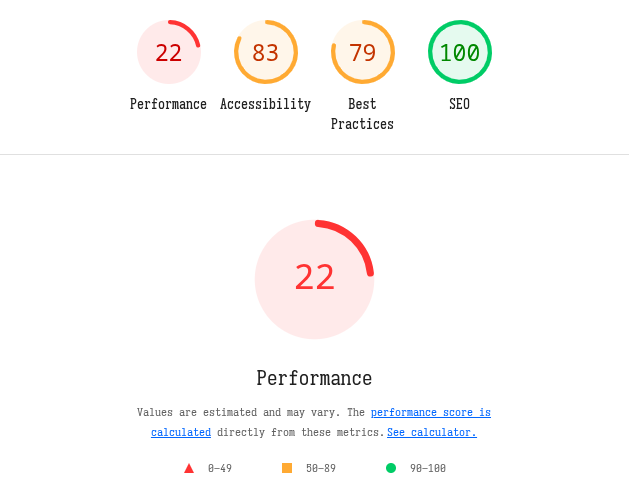
\includegraphics[width=0.8\textwidth]{Imagenes/Bitmap/lighthouse_wuolah.png}
    \caption{Análisis del rendimiento de Wuolah.com con Google Lighthouse.}
    \label{fig:lighthouse}
\end{figure}

La plataforma obtiene una puntuación de rendimiento de 22 sobre 100, un valor que muestra un gran problema de optimización y explica la lentitud que se siente al usarla. Esta baja puntuación se puede explicar por el uso de arquitecturas pesadas en el lado del cliente y la gran cantidad de anuncios que se cargan en este. Esto empeora significativamente la experiencia del usuario y demuestra la necesidad de un enfoque de diseño más eficiente.

El sistema de incentivos que tienen plataformas como Wuolah, basado en micropagos por descarga, presenta un problema de diseño fundamental. Al introducir una recompensa económica, aunque sea mínima, se corre el riesgo de transformar la motivación de los usuarios; el deseo genuino de ayudar es reemplazado por un interés transaccional de bajo valor. Este enfoque se ha demostrado que puede llegar a ser contraproducente. La investigación sobre la motivación ha demostrado que las recompensas externas pueden disminuir el interés propio por realizar una tarea, un efecto conocido como "Desplazamiento Motivacional" \citep{Deci1999, Frey2001}.

Además, este modelo de incentivos tiene una segunda consecuencia negativa para las carreras técnicas. Al limitar las recompensas a los archivos PDF, ya que en estos es en los que se puede incrustar anuncios, se desincentiva a que los estudiantes compartan información en otros formatos más adecuados para ciertas áreas como puede ser en el caso de código empobreciendo así la variedad y utilidad de los recursos disponibles en la plataforma.

Este trabajo busca solucionar todos estos problemas y tiene como objetivo el diseño y desarrollo de un prototipo de plataforma alternativa. La solución propuesta mejorará el rendimiento usando una arquitectura ligera y eficiente usando un backend en Go y un frontend con SvelteKit. Para reducir los costes de mantenimiento se usarán servidores privados virtuales, VPS, en vez de soluciones \textit{serverless} como AWS. Y se eliminará la publicidad invasiva y los incentivos monetarios para fomentar la colaboración genuina y la compartición de recursos en múltiples formatos.

\section{Objetivos}
Descripción de los objetivos del trabajo.


\section{Plan de trabajo}
Aquí se describe el plan de trabajo a seguir para la consecución de los objetivos descritos en el apartado anterior.



\section{Explicaciones adicionales sobre el uso de esta plantilla}
Si quieres cambiar el \textbf{estilo del título} de los capítulos del documento, edita el fichero \verb|TeXiS\TeXiS_pream.tex| y comenta la línea \verb|\usepackage[Lenny]{fncychap}| para dejar el estilo básico de \LaTeX.

Si no te gusta que no haya \textbf{espacios entre párrafos} y quieres dejar un pequeño espacio en blanco, no metas saltos de línea (\verb|\\|) al final de los párrafos. En su lugar, busca el comando  \verb|\setlength{\parskip}{0.2ex}| en \verb|TeXiS\TeXiS_pream.tex| y aumenta el valor de $0.2ex$ a, por ejemplo, $1ex$.

TFGTeXiS se ha elaborado a partir de la plantilla de TeXiS\footnote{\url{http://gaia.fdi.ucm.es/research/texis/}}, creada por Marco Antonio y Pedro Pablo Gómez Martín para escribir su tesis doctoral. Para explicaciones más extensas y detalladas sobre cómo usar esta plantilla, recomendamos la lectura del documento \texttt{TeXiS-Manual-1.0.pdf} que acompaña a esta plantilla.

El siguiente texto se genera con el comando \verb|\lipsum[2-20]| que viene a continuación en el fichero .tex. El único propósito es mostrar el aspecto de las páginas usando esta plantilla. Quita este comando y, si quieres, comenta o elimina el paquete \textit{lipsum} al final de \verb|TeXiS\TeXiS_pream.tex|

\subsection{Texto de prueba}


\lipsum[2-20]